\section{ Hitman Código 47}

\begin{figure}[htbp]
\begin{center}
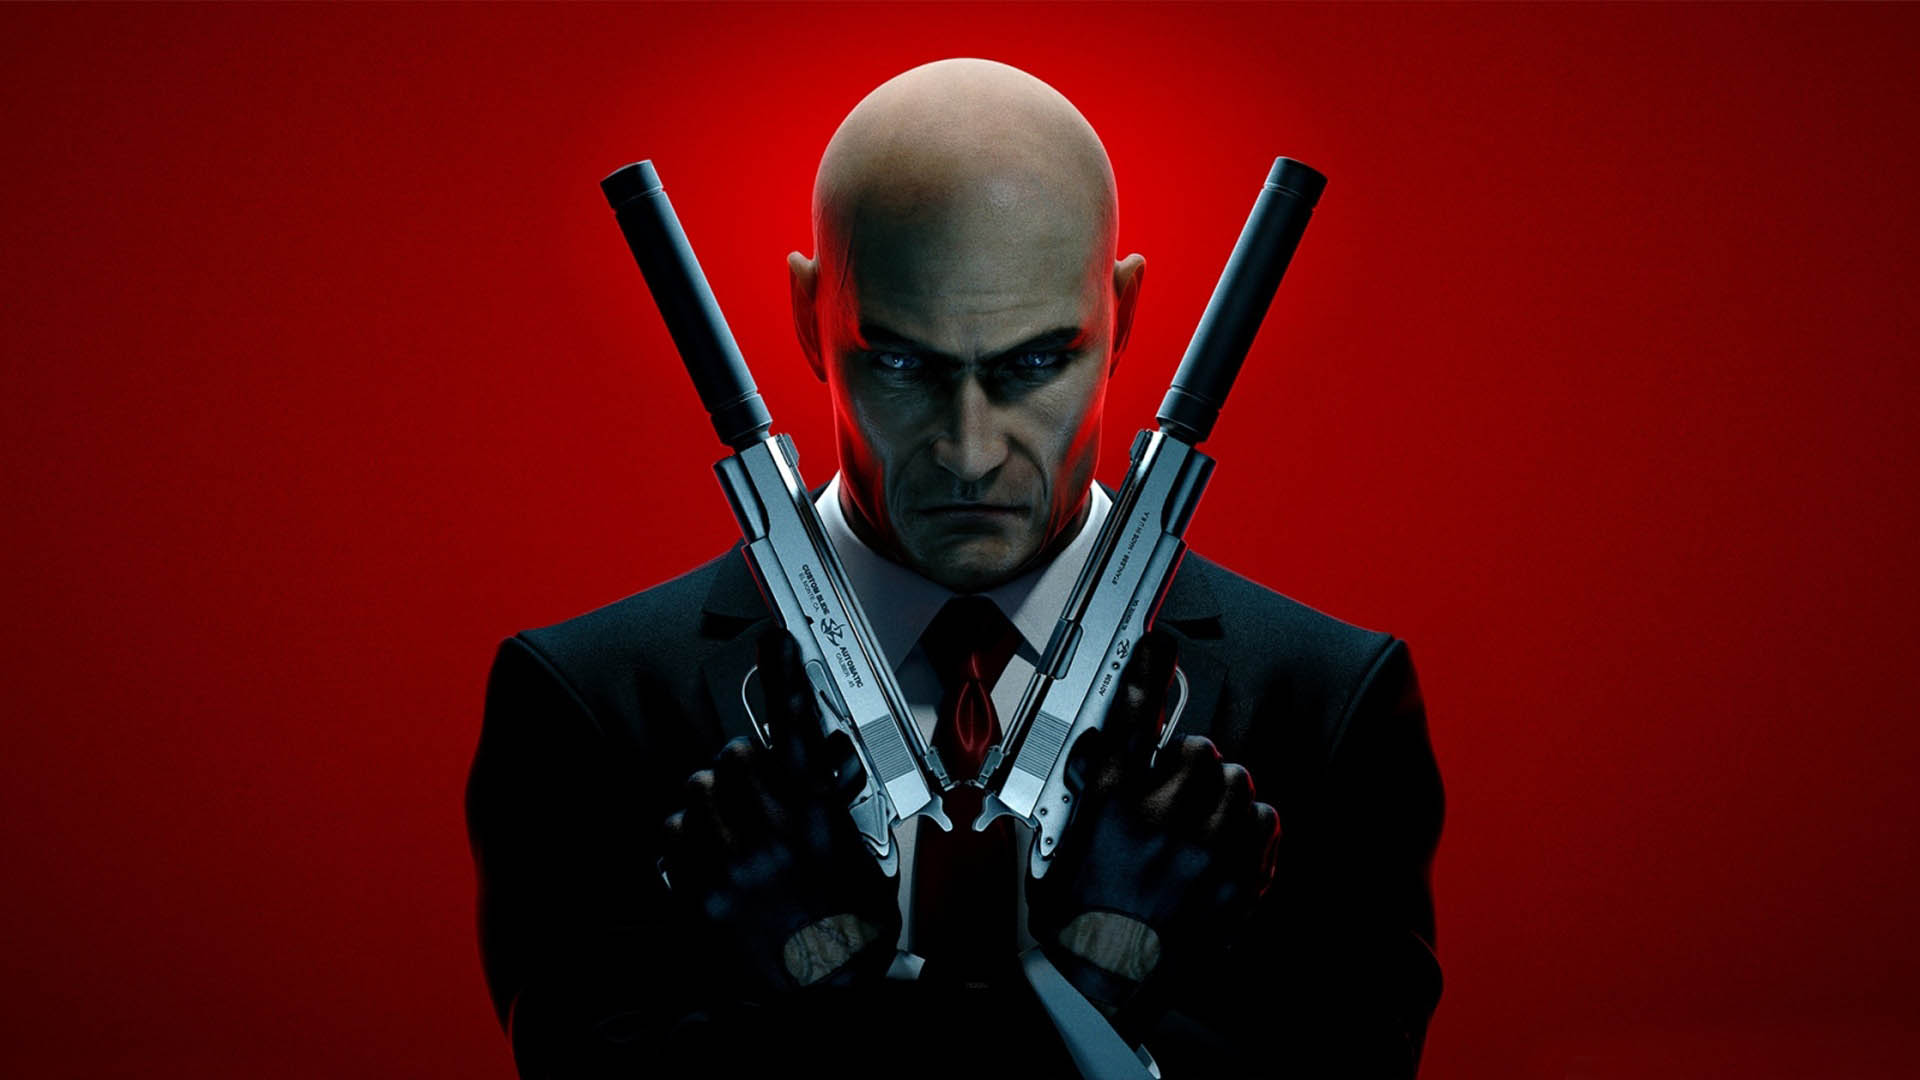
\includegraphics[width=.60\textwidth]{./imagenes/hitman.jpg}
\caption{ Hitman Código 47}
\label{ Hitman Código 47}
\end{center}
\end{figure}
Castlevania\footnote{\url{http://www.guiamania.com/page.php?v=011518/}} es un videojuego de disparos en tercera persona creado por la compañía IO Interactive y publicado por Eidos Interactive en 2000. Es el primer videojuego de la saga de Hitman. Como en todos los juegos de la saga, el personaje principal es el Agente 47, un sicario que trabaja para la ICA (International Contract Agency, Agencia Internacional de Contratos), se divide en varias historias principales, cada una con sus niveles. Antes de cada nivel, la Agencia le da la oportunidad al jugador de seleccionar algunas de las armas y el equipo que va a llevar consigo a la misión, según el dinero que haya obtenido en las anteriores fases. Una vez estudiados los informes de cada objetivo, así como las fotos o los mapas que le puedan ser proporcionados, el jugador inicia la misión. El jugador maneja al propio 47, asesino a sueldo muy habilidoso y sigiloso. En esta, como en todas las entregas de la saga, se castigan los asesinatos de civiles, ya sean peatones, meseros u otros, y lo hace descontando dinero al final de la misión, pudiendo ser considerada fallida si el balance económico es desfavorable para el protagonista. Es por esto que no es un juego en el que la táctica principal sea el enfrentamiento directo con el oponente y matar a diestra y siniestra. Es el engaño y el sigilo la principal arma con que el jugador cuenta. Desde no cargar armas a la vista u obtener información de los personajes con que interactúa hasta otras más sofisticadas, como matar silenciosamente (con una cuerda de piano o un cuchillo) esperando el momento de encontrarse a solas con el objetivo o disfrazarse con las ropas de alguna víctima, son ejemplos de las características del juego. Añadido a eliminar a los objetivos de cada misión, 47 deberá realizar otras tareas secundarias, como esconder cadáveres, desactivar bombas, o liberar inocentes; algunos de ellos le darán información valiosa para el transcurso de la misión..

\subsubsection{¿Por qué es uno de mis juegos favoritos?}
\begin{itemize}
\item[Juan Mite]  Fue la primera parte de una serie de juegos de este asesino a sueldo. Las graficas eran muy buenas para la epoca en que se lanzo debe ser por eso que me impactó.  La trama a simple vista puede ser algo simple (un simple asesino) pero las misiones no son triviales excepto las primeras.  A medida que completes misiones el juego se pondrá más difícil puesto que los blacos tienes mas seguridades varían entre: Diputados, Narcotraficantes, Presidentes, Senadores, Jefes de carteles. 
\end{itemize}
